% What are the typical methods for image segmentation?
\section{Image Segmentation}
When we talk about "Image Segmentation", what exactly are we talking about? Suppose we have a picture of two birds; the segmentation task, or more precisely the \textbf{"semantic segmentation"} task, is to separate the whole image into different regions with different colour codes, where the regions represent the exact position of birds covered on the image and the background. 
\subsection{More on Semantic Segmentation}
The word "semantic" means we always assign a word label (a \textbf{semantic meaning}) to the segmented region, representing what this region refers to. For example, for the example we mentioned above, the regions we segmented for the bird will be assigned with the label "bird", and the background region will be labelled as "background".

\begin{note}
    Semantic segmentation is different from the tasks based on "pure" clustering of images to coherent regions. The regions we are looking to have their value or semantic meaning from the task we defined.
\end{note}
\begin{figure}[H]
    \centering
    \begin{subfigure}[b]{0.47\textwidth}
        \centering
        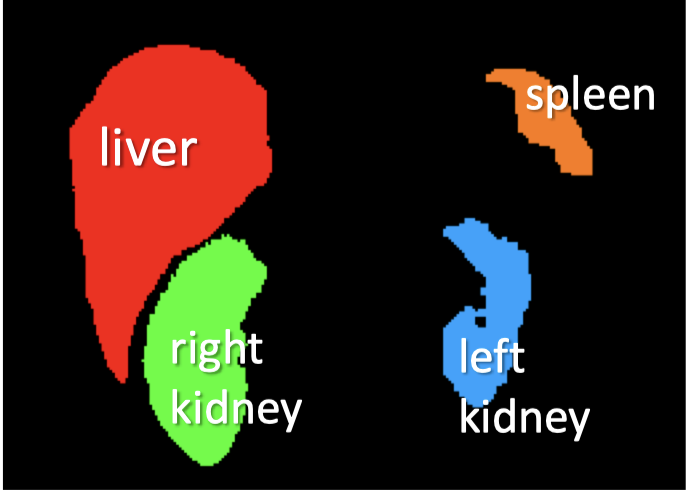
\includegraphics[width=\textwidth]{./figures/semantic-segmentation.png}
        \caption{Semantic Segementation}
        \label{fig:semantic-segmentation}
    \end{subfigure}
    \hfill
    \begin{subfigure}[b]{0.47\textwidth}
        \centering
        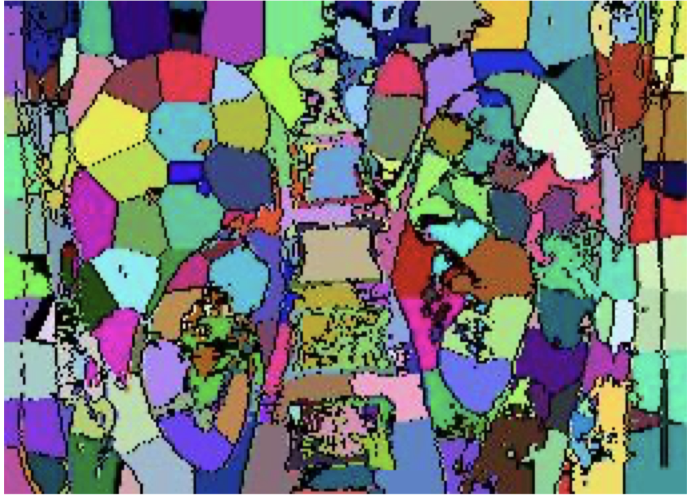
\includegraphics[width=\textwidth]{./figures/clustering.png}
        \caption{Segmentation based on clustering}
        \label{fig:normal-segmentation}
    \end{subfigure}
       \caption{Different Image Segmentation Tasks}
       \label{fig:segmentations}
\end{figure}
\noindent After getting a glance at \textbf{Semantic Segmentation}, we will discuss the methods for segmentation tasks in the following sections.
\section{Manual Segmentation}

Manual Segmentation must be the most straightforward method we can come up to our mind. It refers to a process that lets human experts as an observer make gold standard labels based on their background knowledge. It is clear to see that the segmented labels are confirmed to be validated. However, it might take a long time for human observers to create such labels due to the time cost of training and the amount of data required to be labelled. \medskip

\noindent Furthermore, inter or intra-observer variability may bring a concern to the validity of the labelled data by manual segmentation since there might be disagreement between different human observers and/or disagreement from one observer but on different occasions. Also, the bias from human experts might cause problems. We still need the assistance of computers to utilise intelligence for performing the segmentation task. 

\section{Threshold-based Methods}

Thresholding is one of the simplest and most popular segmentation techniques used in the industry. This method is based on the assumption that intensity distribution has multiple modes. That is to say, the grayscaled intensity of the pixels can be divided into two (or more) clusters, and we can pick thresholds from the "gaps" between the clusters to segment the background and foreground. The segmentation can be achieved by setting the pixels with an intensity lower than the threshold background and those with an intensity equal to or greater than the threshold foreground. It is also accepted to select multiple thresholds to select pixels within a specific range only for segmentation. \medskip

\noindent The algorithm is simple and fast, yet the algorithm can only be applied when regions (of interest) are homogeneous and distinct. That is to say, the pixels in the same region should have similar intensity values. Also, finding consistent threshold frequencies across different images is different, since the intensity of pixels will vary from image to image.
\section{Region-based Methods}
The region-growing method is a typical region-based method. The algorithm is based on the assumption that the segmented regions are homogeneous. The algorithm starts with a seed pixel, and then it will grow the region by adding pixels similar to the seed pixel. The algorithm will stop when the region reaches a specific size or when the region is homogeneous, where interpreted as the neighbouring pixels are too dissimilar with each other in comparison \cite{adams1994seeded}. \medskip

\noindent Applying the region-growing method is usually very efficient, yielding a connected region from the seed point. Unlike thresholding, region-growing methods achieve segmentation without the explicit use of image properties. However, the region-growing method is not robust to noise since the algorithm will keep growing the region even if the neighbouring pixels are not similar to the seed pixel. \medskip

\noindent Another major issue that the region-growing method has is that the initial seed point selection is significant. If the seed point is not selected correctly, the algorithm will not be able to grow the region properly. Consequently, this initial step is time-consuming and inaccurate to find the optimal seed point, and it also requires human intervention to evaluate the choice of seed point. \medskip

\noindent To address this problem in medical imaging, Poonguzhali et al. proposed an automatic region growing method for ultrasound images \cite{poonguzhali2006complete}. They adopt an automatic seed point selection based on textural features such as co-occurrence features and run length features without human intervention. The experimental results showed the feasibility and effectiveness of the proposed region-growing algorithm in selecting seed points and segmenting the ROI without manual intervention.\medskip

\section{Deep Learning Methods}
U-Net \cite{ronneberger2015u} is a deep learning method for image segmentation. It is a fully convolutional network (FCN) \cite{long2015fully} that uses a contracting path to capture image context and a symmetric expanding path that enables a precise level of localization. The network is trained end-to-end from raw pixels to pixel-wise segmentation masks. The network architecture is shown in \autoref{fig:unet}. \medskip
\begin{figure}[H]
    \centering
    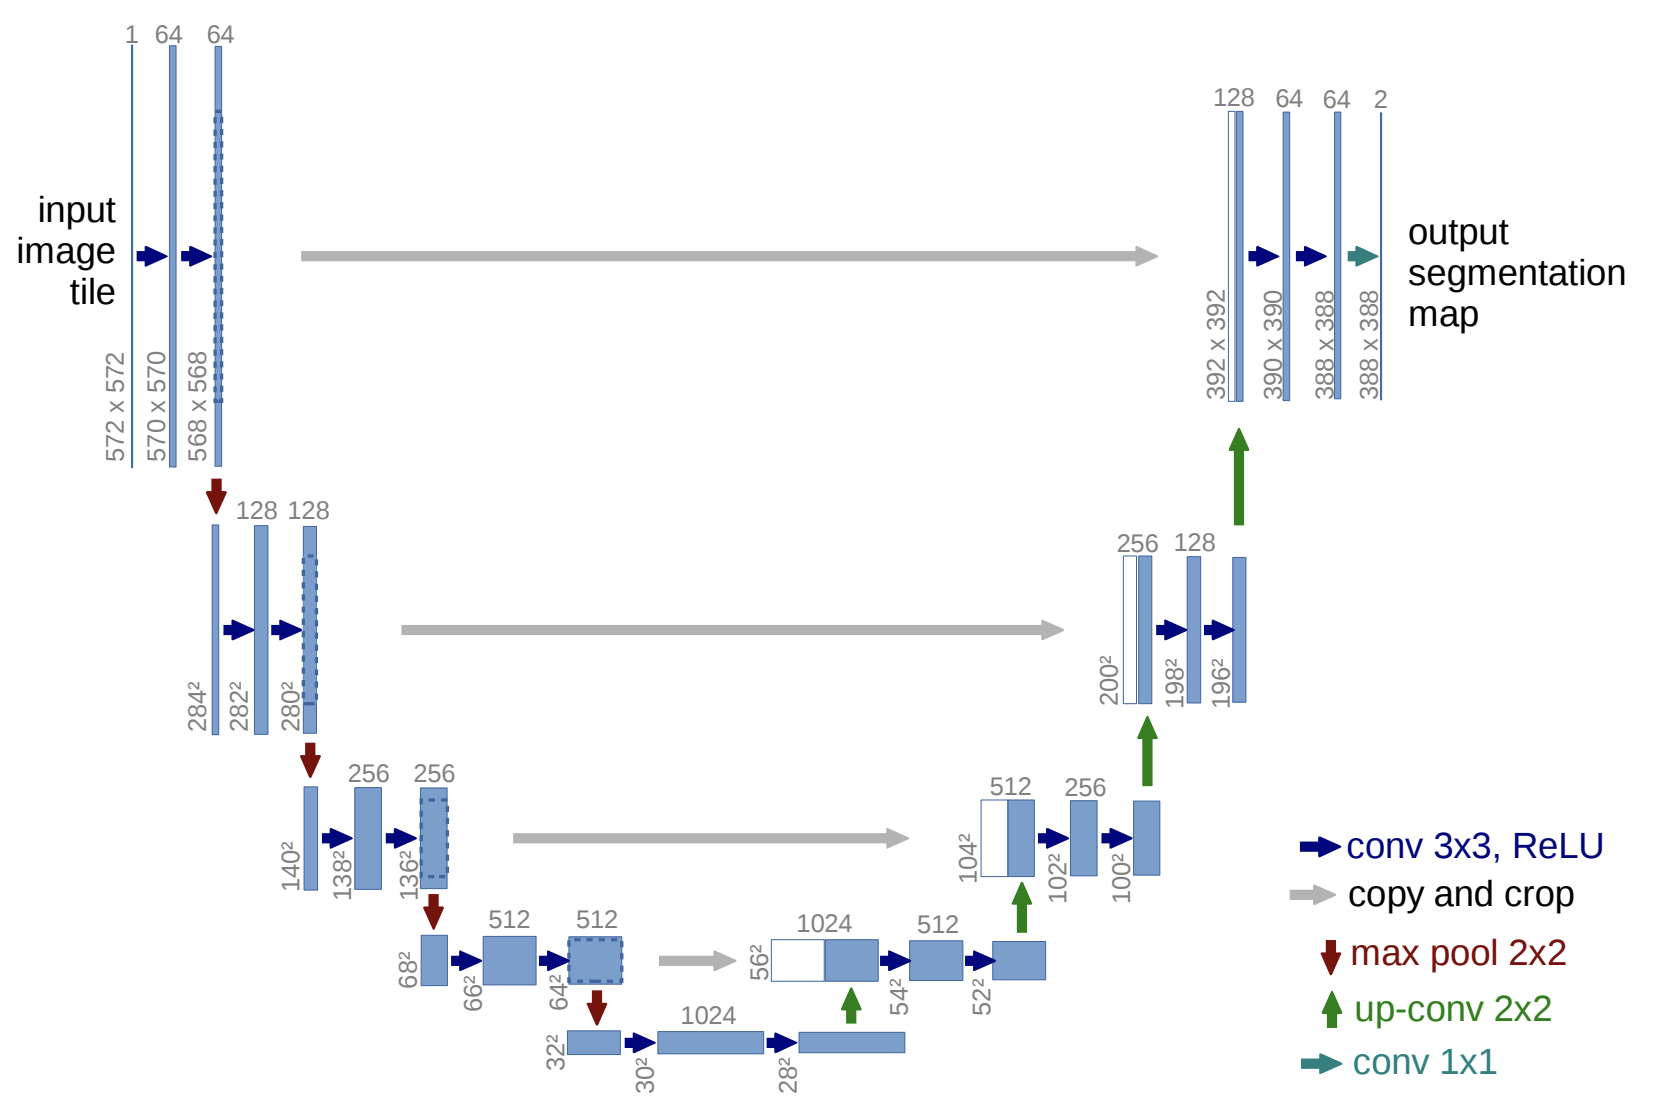
\includegraphics[width=0.8\textwidth]{./figures/unet.png}
    \caption{An example of the U-net architecture. Each blue
    box in the figure represents a multi-channel feature map, and on the top of each box indicates the number of channels. The \(x\)-\(y\)-size is shown at the lower left edge of the box. Each white box represents a copied feature maps. The arrows denote the different operations.}
    \label{fig:unet}
\end{figure}
\noindent In the contracting path of the network (on the left), the network consists of a series of repeated applications. Each step starts with two 3x3 convolutions, and each convolution doubles the number of feature maps. Then the network applies a rectified linear unit (ReLU) as activation, followed by a downsampling step via a 2x2 max pooling operation with a stride of 2. \medskip

\noindent The expansive path (on the right) starts with an upsampling of the feature map followed by a 2x2 convolution, halving the number of feature channels. The feature maps are then concatenated with the corresponding crops of the contracting path. After that, two 3x3 convolutions are applied to the image, and a ReLU activation follows each convolution. The reason for cropping the convolution results from the contraction path is the loss of border pixels in every convolution. At the final layer, the network used a 1x1 convolution to map each 64-component feature vector to the desired number of classes. \medskip

\noindent nnU-Net \cite{isensee2021nnu}, a framework based on U-Nets, is a self-configuring segmentation framework that can automates the configuration of the preprocessing, network architecture, training, and post-processing of a segmentation pipeline. The selected configuration is depending on the medical data used for training. The framework provides a fully automated segmentation workflow that can be trained and inferred on any medical dataset. \medskip

\noindent For deterimining hyperparameters, nnu-Net uses "data-fingerprints" with heuristic rules to select the best hyperparameter configuration for a given dataset before processing the training data. The framework also uses data fingerprints to generate pipeline configurations including the inferred parameters (image resampling, normalisation, batch, and patch size), and the blueprint parameters (loss function, optimiser, architecture). \medskip

\noindent Combined with pre-selected hyperparameters and the pipeline configurations, the pipeline generates network training for 2D, 3D full-resolution, and 3D-Cascade U-Nets \cite{isensee2018nnu}. The optimal performance (e.g. average dice coefficient) is obtained by ensemling the configurations of the three networks. After that the optimal configuration will be deployed and evaluated on test dataset. The pipeline architecture is shown below. \medskip

\begin{figure}[H]
    \centering
    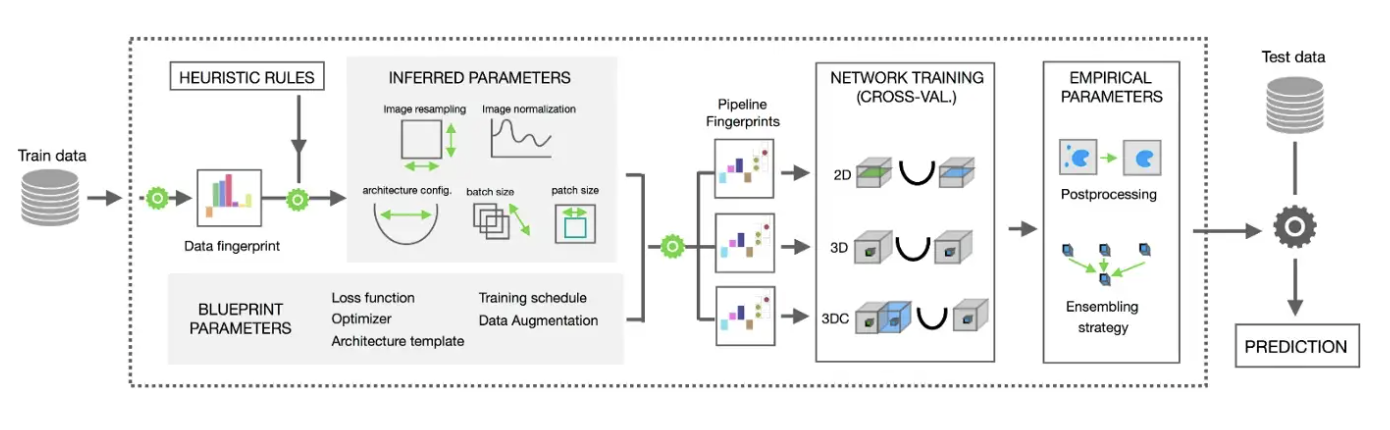
\includegraphics[width=\textwidth]{./figures/nnunet.png}
    \caption{The pipeline representation of nn-UNet.}
    \label{fig:hello}
\end{figure}
\noindent The nnU-Net has achieved the state-of-the-art performance on a variety of medical imaging tasks, including brain tumour segmentation, prostate segmentation, and liver segmentation \cite{isensee2019nnu}. \medskip







